%% main.tex — OUP template (clean, one section per page)
%% ANNOTATED VERSION — Philippine, April 2026
%% Changes are colored:
%%   \new{...}  = blue, new additions
%%   \edit{...} = magenta, modifications to existing text
%% Each colored block is preceded by a comment % [EVAN p.X] or % [PB note N]
%% To remove all colors later: replace \new and \edit with identity macros.

\documentclass[unnumsec,webpdf,modern,mediumone]{oup-authoring-template}

\graphicspath{{Fig/}}

% -----------------------------
% Line numbers
% -----------------------------
\usepackage[mathlines,switch]{lineno}

\usepackage{etoolbox}
\usepackage{tikz}
\usetikzlibrary{arrows.meta, positioning, calc}

% -----------------------------
% Reduce layout overflow issues
% -----------------------------
\raggedbottom

% Math (safe)
\usepackage{amsmath,amssymb}
\usepackage{pifont}

% -----------------------------
% Revision-tracking macros
% -----------------------------
\usepackage{xcolor}
% Using color groups ({\color{...}...}) rather than \textcolor{...}{...}
% so the macros can span paragraph breaks, list environments, etc.
\newcommand{\new}[1]{{\color{blue}#1}}
\newcommand{\edit}[1]{{\color{magenta}#1}}
% To clear all highlighting before submission, replace the two lines above with:
%   \newcommand{\new}[1]{#1}
%   \newcommand{\edit}[1]{#1}

\begin{document}

\journaltitle{Journal of the Royal Statistical Society: Series A}
\DOI{DOI added during production}
\copyrightyear{2026}
\pubyear{2026}
\vol{XX}
\issue{x}
\access{Submitted: January 2026}
\appnotes{Paper}

\firstpage{1}

\title[MLE for Intermittent Methane Emissions]{Maximum Likelihood Estimation of Intermittent Methane Emissions from Heterogeneous Monitoring Data}

\author[1,$\ast$]{Philippine Burdeau}
\author[2,3]{Evan Sherwin}
\author[1]{Adam Brandt}

\address[1]{%
\orgdiv{Department of Energy Science \& Engineering},
\orgname{Stanford University},
\orgaddress{\country{USA}}}

\address[2]{%
\orgdiv{Systems and Energy Technologies Analysis Department},
\orgname{Lawrence Berkeley National Laboratory},
\orgaddress{\country{USA}}}

\address[3]{%
\orgdiv{Integrated Ecosystem Sciences Department},
\orgname{Lawrence Berkeley National Laboratory},
\orgaddress{\country{USA}}}

\corresp[$\ast$]{Corresponding author.
\href{mailto:pburdeau@stanford.edu}{pburdeau@stanford.edu}}

\abstract{
Methane point-source monitoring relies on an expanding array of technologies, from satellites and aircraft to mobile surveys and continuous ground-based sensors. Because emissions are intermittent, repeated observations of the same facility may sample the same underlying emission event, making observations statistically dependent. Existing approaches treat each observation as statistically independent, discarding this temporal structure and inflating estimation variance. We develop and present a maximum likelihood framework that jointly models emission dynamics and the observation process to incorporate this dependence. The method represents latent emission states as a Markov chain, corrects for size-dependent detection bias via inverse-probability weighting, and extracts information from both detections and non-detections across technologies with different sensitivities and sampling cadences. In simulations calibrated to intensive monitoring scenarios combining continuous sensors with snapshot observations, the method achieves approximately \edit{38}\% variance reduction relative to the standard POD-weighted estimator under baseline conditions, with larger gains for persistent emissions. Actual variance reduction in real-world surveys will depend on characteristics of the underlying emissions system, which is currently poorly understood due to limited comprehensive survey data from around the world. However, robust benefits in variance under many simulated conditions suggests that this method will likely result in improved estimates.
}


\keywords{methane emissions, intermittency, maximum likelihood estimation,
detection probability, irregular sampling, hidden Markov model}

\maketitle

% Line numbers start AFTER title/abstract
\linenumbers
% Introduction Draft — February 2026

\section{Introduction}
\label{sec:introduction}

% --- What problem / Why important ---

Methane is the second-largest driver of anthropogenic climate forcing, responsible for roughly 30\% of the rise in global mean temperature since the pre-industrial era \citep{IPCC2021}. Because of its short atmospheric lifetime ($\sim$12 years), methane mitigation yields climate benefits on a decadal timescale that CO\textsubscript{2} abatement alone cannot deliver \citep{Ocko2021}. The oil and gas sector accounts for 20--25\% of global anthropogenic methane emissions \citep{Saunois2020, Saunois2025}, and actual emissions appear to substantially exceed official inventories \citep{Alvarez2018, Brandt2014}, so these estimates may undercount the importance of oil and gas as a methane source. Accurate methane emission estimates are critical to inform regulation and to effectively target mitigation. A growing number of measurement technologies can be used to detect and quantify these emissions. However, each methane sensing technology can have varying detection and quantification performance, and the problem we address is how to estimate total emissions from the heterogeneous and complex data that such sensors produce.


% --- Why it is hard ---

This estimation problem is hard because it involves two fundamentally distinct sources of uncertainty: uncertainty in the emission process and uncertainty in the measurement system. These uncertainties can interact in difficult-to-interpret ways. For example: if a previously detected emission source is not seen in a follow-up survey, does that mean that the emission stopped, or was the emission simply not detected due to an emission rate in the methane sensing system's partial detection range?

% --- Emission uncertainty ---

On the emission side, two features make the problem challenging. First, site-level emissions are sometimes intermittent. Equipment such as compressors, tanks, and flare systems cycles between emitting and non-emitting states on timescales ranging from minutes to weeks \citep{Cusworth2021, Daniels2024}. \citet{Cusworth2026NatComms} classified super-emitter events in the Permian Basin into finite (median duration 2.4--145 hours), mixed (semi-bounded), and unbounded categories, illustrating the wide range of temporal behaviors at play. Different datasets seem to suggest different values for duration distributions of emissions. Thus, a facility that is emitting during one observation may be inactive during the next, and vice versa. Second, emission rates can vary widely: when a facility does emit, its instantaneous rate is not a fixed value but can possibly vary over several orders of magnitude across time. Emissions distributions on the whole typically follow a right-skewed, heavy-tailed distribution, but it is unclear what fraction of this variance would be observed in a single emission source varying over time \citep{Brandt2014, ZavalaAraiza2015, Brandt2016, Duren2019}. Very few (if any) datapoints in the public literature look at single leaks in detail over long time periods, making this an important source of uncertainty.

% --- Measurement uncertainty ---

On the measurement side, two challenges introduce additional complexity. First, the sampling process varies widely across technologies, in both its temporal and spatial dimensions. Satellites can measure anywhere in the world, in some cases providing global spatial coverage, but high-sensitivity tasked systems do not necessarily revisit individual facilities frequently \citep{Jacob2022, Jervis2025Science}, creating an effectively ``snapshot'' view of emissions over seconds while the satellite passes over. Their ability to pinpoint the source of a leak is limited to resolution of (order of magnitude) 10-100 m at the finest resolution. Many instruments exist that only provide km-scale spatial resolution. Airborne imagers also create snapshot images of emissions due to relatively high flight speed. Spatially, they cover smaller areas at higher spatial resolution \citep{Cusworth2026NatComms, Sherwin2024Nature}. They can more closely pinpoint leak location and detect smaller emissions, typically with higher costs per facility scanned due to airplane and pilot costs. Mobile ground surveys offer fine spatial detail along driven routes \citep{Omara2018}, but require inverse modeling to infer source location from detection data, and can only sample near the ground, potentially missing lofted plumes. Continuous monitoring systems produce dense time series at fixed locations but are subject to wind-direction gaps due to changing weather conditions \citep{Daniels2024}. The result is that these different instruments sample the emission process at very different temporal and spatial scales. 

Second, all measurements are subject to error. Instruments fail to detect some emissions, with a probability of detection (POD) that depends on emission rate \citep{Sherwin2021, Sherwin2023}. The POD for each technology is only partly understood and may differ between structured blind tests and real-world deployments. And once emissions are detected, quantification algorithms come with substantial uncertainty \citep{Sherwin2023, Wigle2024}. In some technologies, this uncertainty appears as quantification bias, while other technologies are relatively unbiased but exhibit significant noise in quantified emission rate estimates.

% --- Why existing approaches are not sufficient ---

A growing body of work has seeks to estimate facility-level or regional emissions from measurements \citep{Sherwin2024Nature, Jervis2025Science, Johnson2023CommEE, Cusworth2021}. A key line of research concerns correcting for detection bias. Because POD rises gradually with emission rate, an uncorrected sample of detected plumes under-represents the left tail of the true distribution. Several influential studies have characterized emission distributions or estimated regional totals directly from detected plumes without explicitly modeling the POD \citep{Lauvaux2022, Ehret2022, Frankenberg2016}. Recognition of this bias has spurred a growing effort to account for it. Controlled-release experiments have characterized POD curves for individual sensors \citep{Sherwin2021, Bell2022, Conrad2023, ElAbbadi2024, GHGSatMATM2025}, and various corrections have been proposed: scaling detected rates by detection frequency \citep{Jervis2025Science}, splicing simulated distributions below a threshold \citep{Sherwin2024Nature}, or partitioning emissions into measurable and unmeasurable components \citep{Johnson2023CommEE}. Most recently, \citet{JervisPreprint2025} jointly estimated a lognormal emission-rate distribution and a continuous POD function via maximum likelihood, without relying on controlled-release calibration. This approach operates at the population level across facilities and treats all plume detections as independent draws.


% [EVAN p.3 — "This is partially true. We should cite the recent Conrad & Johnson paper looking at the impact of..."]
The assumption of independence underlies a second limitation: current methods do not accurately account for temporal dependence. Existing estimation methods are typically designed around a single instrument and treat successive revisits as exchangeable. The simplest approach, and a natural one for a single sensor with regular cadence, is to compute the empirical mean over repeated visits including non-detections. This implicitly accounts for intermittency and yields a valid time-averaged rate, as done by \citet{Chen2022EST} and \citet{Sherwin2024Nature}\new{; recent work by \citet{Conrad2023} further examines the impact of revisit structure on such estimates}. Some approaches do not handle this issue correctly. For example, \citet{Williams2025ACP} compute such a mean and then multiply by a separately estimated persistence fraction, double-counting intermittency. No current method, however, accounts for the temporal correlation between successive observations. This correlation is particularly important when combining data from instruments with very different revisit cadences. Other such issues arise with sensors where measurements are highly ``clumped'' in time, such as a regional airplane survey done over a few days or weeks, with no additional measurements taken for months or years. Not accounting for such correlation inflates the variance of the resulting estimate beyond what the sample size alone would suggest.

% [EVAN p.5 — "How does treating redundant observations as independent increase variance, rather than decrease it?"]
% [PB note 1 — correlated-samples variance result; detailed derivation moved to SI]
\new{The cost of ignoring this correlation is quantifiable. When repeated observations sample the same persistent emission event, they carry overlapping information rather than independent draws, and an estimator that averages them as if they were independent is strictly sub-optimal: its variance exceeds what an estimator that accounts for the correlation structure could achieve. The gap widens as observations become more tightly correlated, and vanishes only in the limiting case of independent samples. A formal derivation is given in SI, Section~\ref{sec:corr_mean_SI}. The MLE we develop below recovers this otherwise-discarded information by explicitly modelling the source of correlation, namely the latent emission state.}

Lastly, stochastic simulation studies have modeled intermittency at the single-facility level \citep{Hodshire2025}, but only as a forward problem. This modeling approach is useful for simulation in cases where we ``know'' the underlying distributions of emissions from which to draw, but does not allow us to take sets of new real-world observations into account when creating a new picture of the true underlying data distribution. This inferential problem is what we are concerned with here.



% --- What we do ---

Our improved method accounts for an important feature of this problem: Detection bias and temporal dependence interact because whether a non-detection reflects the lack of an emission or a missed emission depends on the surrounding observation history (Figure~\ref{fig:challenges}). Addressing both requires a joint model of the emission dynamics and the measurement process. We develop such a model here, based on maximum likelihood estimation (MLE). The emission process is modeled as a stationary two-state Markov model, capturing intermittency, with a log-normal distribution for the emission rate when active, capturing the heavy-tailed randomness of emission sizes. The measurement processes are specified through POD curves and noise models. Together, these define a likelihood over the full observation sequence, from which the time-averaged emission rate follows as the product of the stationary ON-state probability and the conditional mean emission rate. Under standard regularity conditions, the MLE is asymptotically unbiased and has lower variance than linear estimators \citep{vanderVaart1998}.

Our main contribution is the framework itself. \edit{The framework is deliberately agnostic to the underlying measurement technology: a sensor enters the likelihood through three modular inputs — its probability-of-detection curve, its noise model, and its sampling cadence — all of which are observable or estimable from controlled-release data or deployment logs. Nothing in the estimator depends on whether the underlying platform is a satellite, an aircraft, a mobile ground survey, or a fixed fenceline sensor, and new instruments can be added to an existing analysis by specifying these three components without structural changes.} % [EVAN: strengthen tech-agnostic framing]
This modularity is what enables principled fusion of heterogeneous data at the same facility, and matters increasingly as the monitoring landscape diversifies. \edit{We develop the framework here for the canonical case of a single facility observed over time; multi-source spatial aggregation poses distinct modeling challenges — principally the specification of a joint emission model — that we leave to future work.}

% [EVAN p.12 — "I recommend highlighting this general point in the introduction. Readers may not immediately understand..."]
\new{These variance gains translate directly into reductions in the sample sizes required by monitoring programs. Because the number of site-visits needed to reach any precision target scales linearly with estimator variance, the roughly 38\% variance reduction we report below reduces the required sample size by the same fraction. For operators surveying many facilities, this corresponds to either narrower confidence intervals at fixed expenditure or lower expenditure at fixed precision; for regulators, it expands the set of emission changes that can be resolved above sampling noise. We quantify these implications in Section~\ref{sec:results}.}

The remainder of the paper proceeds as follows. Section~2 presents the model and estimation framework. Section~3 describes the simulation experiments and reports results. Section~4 discusses implications, limitations, and extensions. Section~5 concludes.


\newpage
\section{Model and Estimation Framework}
\label{sec:methods}

This section presents our statistical model for intermittent emissions observed by heterogeneous technologies (Section~\ref{sec:stat_model}) and the estimation procedure that jointly infers emission dynamics and corrects for detection bias (Section~\ref{sec:estimation}).

% [PB note — terminology standardization up front, addressing several Evan comments:
%   "Is a release different than an emission?" (p.4),
%   "What does 'observation unit' mean?" (p.12),
%   "How many hours are in a time step?" (p.6),
%   "What constitutes a campaign?" (p.12)]
\new{\paragraph{Terminology.}
Throughout the paper we use ``emission'' to refer to a period of active methane release from a source; ``release'' appears only in the specific context of controlled-release experiments, where it refers to a deliberately injected test plume. A ``time step'' denotes the discrete unit of the simulated Markov chain; in all numerical experiments we fix it at one hour, chosen to match the characteristic timescale of operational equipment cycles and of atmospheric variability seen by continuous monitors. A ``campaign'' is the full monitoring record over the analysis window $T$ for a single source; it may contain zero, one, or many snapshot visits and zero or more continuous-monitoring windows.}

\begin{figure}[htbp]
\centering
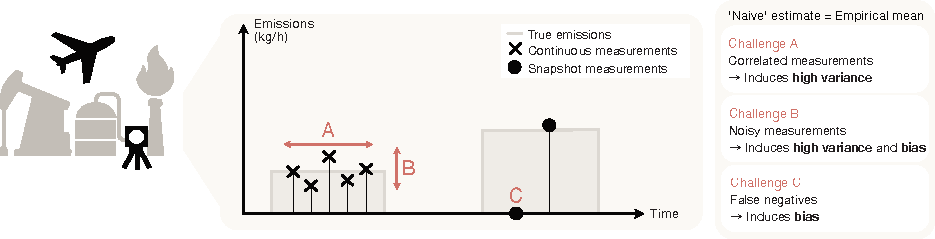
\includegraphics[width=\textwidth]{figures/figure0.pdf}
\caption{Conceptual overview of the estimation challenges. An intermittent source switches between active and inactive states over time. Continuous monitors (crosses) and snapshot measurements (circles) sample this process irregularly. Three challenges arise: \textbf{(A)}~multiple measurements may observe the same emission event, resulting in correlated measurements; \textbf{(B)}~detected emissions are measured with noise, increasing the variance of and potentially introducing biases on naive estimates; \textbf{(C)}~small emissions fall below the detection threshold, producing false negatives that bias the observed sample toward large values. Our framework addresses these challenges jointly.}
\label{fig:challenges}
\end{figure}

\subsection{Statistical Model}
\label{sec:stat_model}

We model the data-generating process as a four-layer hierarchical process (Figure~\ref{fig:model_overview}). First, a latent ON/OFF state governs whether the source is emitting. Next, when the emission is active, the emission rate is drawn from a continuous distribution at event onset and persists at a constant rate until the event ends. Third, the observation process then filters this signal through sensor-dependent detection probability. And fourth, the size of the emission is estimated with possible quantification noise. A key estimation challenge is that detection probability depends on emission size, so non-detections are ambiguous: they may reflect true inactivity or a missed emission. Our framework addresses this by formally defining the likelihood of the observed sample, decomposing it into tractable components, and optimizing unknown parameters with an iterative strategy.

\begin{figure}[htbp]
\centering
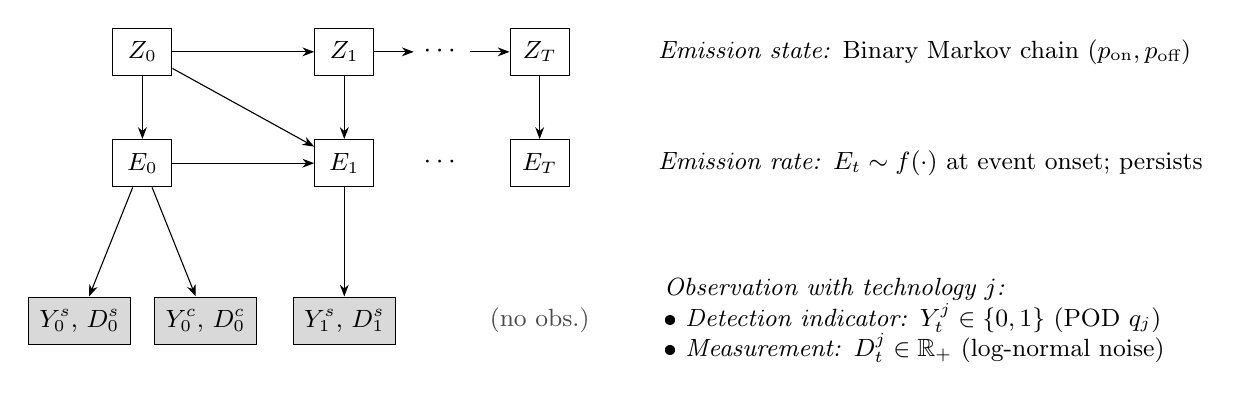
\begin{tikzpicture}[
    node distance=0.8cm and 1.8cm,
    box/.style={draw, minimum width=0.75cm, minimum height=0.6cm, font=\small},
    obs/.style={box, fill=gray!30},
    obswide/.style={draw, fill=gray!30, minimum width=1.3cm, minimum height=0.6cm, font=\small},
    arrow/.style={-{Stealth[length=1.5mm]}},
]
% Layer 1: Emission state
\node[box] (Z0) {$Z_0$};
\node[box, right=of Z0] (Z1) {$Z_1$};
\node[right=0.5cm of Z1] (Zdots) {$\cdots$};
\node[box, right=0.5cm of Zdots] (ZT) {$Z_T$};
\draw[arrow] (Z0) -- (Z1);
\draw[arrow] (Z1) -- (Zdots);
\draw[arrow] (Zdots) -- (ZT);

% Layer 2: Emission rate
\node[box, below=of Z0] (E0) {$E_0$};
\node[box, below=of Z1] (E1) {$E_1$};
\node (Edots) at ([yshift=-1.4cm] Zdots) {$\cdots$};  % explicitly aligned with E0/E1
\node[box, below=of ZT] (ET) {$E_T$};
\draw[arrow] (Z0) -- (E0);
\draw[arrow] (Z1) -- (E1);
\draw[arrow] (ZT) -- (ET);
\draw[arrow] (E0) -- (E1);
\draw[arrow] (Z0) -- (E1);

% Layer 3: Detection + measurement
\node[obswide] (O0s) at ([xshift=-0.8cm, yshift=-2.0cm] E0) {$Y_0^s,\, D_0^s$};
\node[obswide] (O0c) at ([xshift=+0.8cm, yshift=-2.0cm] E0) {$Y_0^c,\, D_0^c$};
\draw[arrow] (E0) -- (O0s);
\draw[arrow] (E0) -- (O0c);

\node[obswide] (O1s) at ([xshift=0cm, yshift=-2.0cm] E1) {$Y_1^s,\, D_1^s$};
\draw[arrow] (E1) -- (O1s);

\node[font=\small, text=gray!60!black] (noobs) at ([yshift=-2.0cm] ET) {(no obs.)};

% Right-side annotations — anchored to exact y of each layer
\node[right=1.0cm of ZT, font=\small, align=left] {%
    \textit{Emission state:} Binary Markov chain $(p_{\text{on}}, p_{\text{off}})$};
\node[right=1.0cm of ET, font=\small, align=left] {%
    \textit{Emission rate:} $E_t \sim f(\cdot)$ at event onset; persists};
\node[right=0.7cm of noobs, font=\small, align=left] {%
    \textit{Observation with technology $j$:}\\
    \textbullet~\textit{Detection indicator:} $Y_t^j\in\{0,1\}$ (POD $q_j$)\\
    \textbullet~\textit{Measurement:}
    $D_t^j\in\mathbb{R}_+$ (log-normal noise)};

\end{tikzpicture}
\caption{Graphical model for intermittent emissions with imperfect detection. Shaded nodes are observed; unshaded nodes are latent. The emission state $Z_t$ follows a two-state Markov chain. The emission rate $E_t$ is drawn at event onset and persists until the event ends. At each time step, the true rate may produce zero, one, or two pairs of detection/measurement outcomes depending on which technologies are deployed: $Y_t^j$ (detection indicator) and $D_t^j$ (measured value) for technology $j \in \{s, c\}$. Here $t = 0$ illustrates a dual-observation time step, $t = 1$ a single-technology observation, and $t = T$ an unobserved time step. When both technologies are present their detections are conditionally independent given $E_t$.}
\label{fig:model_overview}
\end{figure}

\paragraph{Emission process.}
We model an emission source as switching between ON and OFF states over discrete time steps $t = 1, \ldots, T$. Let $Z_t \in \{0, 1\}$ denote the latent (unobserved) state, where $Z_t = 1$ indicates an active emission. The state sequence follows a two-state Markov chain with transition probabilities $p_{\text{on}} = p(Z_t = 1 \mid Z_{t-1} = 0)$ and $p_{\text{off}} = p(Z_t = 0 \mid Z_{t-1} = 1)$. The stationary probability of being ON is $\pi_{\text{on}} = p_{\text{on}} / (p_{\text{on}} + p_{\text{off}})$, and the mean emission duration is $\tau = 1/p_{\text{off}}$ time steps.

% [EVAN p.5 — "What functional form are we assuming for f(e)?"]
When $Z_t = 1$, the emission rate $E_t$ is drawn from an unknown distribution $f(\cdot)$ ($f(e)\doteq p(E_t=e|Z_t=1)$) at the start of each emission event and persists until the event ends. When $Z_t = 0$, $E_t = 0$. \edit{In our simulations we adopt a lognormal specification for $f$, which matches the right-skewed, heavy-tailed behavior observed empirically for oil-and-gas leaks \citep{Brandt2016, ZavalaAraiza2015}. The choice is not critical to the framework: as we show below, the estimation procedure depends on $f$ only through the average detection probability it implies, so the lognormal can be replaced by any nonnegative distribution without modifying the algorithm. Some sites and basins are better described by heavier-tailed or mixture forms \citep{Sherwin2024Nature}, and we discuss the implications in Section~\ref{sec:discussion}.} Our target estimand is the time-averaged emission rate:
\begin{equation}
    \mu 
    \doteq \mathbb{E}[E_t]
    = \mathbb{E}[\mathbb{E}[E_t\mid Z_t]]
    = \frac{p_\text{on}}{p_\text{on}+p_\text{off}}\cdot \mu_\text{emit},
    \label{eq:target}
\end{equation}
where $\mu_\text{emit}\doteq\mathbb{E}[E_t\mid Z_t=1]$.

\paragraph{Observation process.}
Each observation is characterized by three modular components: a detection probability curve, a noise model, and a sampling cadence. Different technologies differ in these three characteristics, and our framework treats them as modular inputs.

The two monitoring technologies have different deployment physics. At each time step $t$, a snapshot observation occurs independently with probability $p_{\text{snap}}$ (modelling discrete aerial or satellite visits). Continuous monitors follow a renewal process: at each unmonitored time step, a Bernoulli draw with probability $p_{\text{cont}}$ triggers deployment of a monitor that then runs for $T_{\text{cont}}$ contiguous time steps; during an active window no new deployment draw is made, and snapshots can still occur. This set of contiguous time steps represents the set of time steps over which the continuous monitoring technology has visibility into the release. For example, as winds change a visible release may become invisible to a continuous monitoring technology.

% [EVAN — justify the renewal process for continuous monitors physically]
\new{This Bernoulli-onset, fixed-duration structure is a coarse abstraction of the physical process governing sensor visibility. Continuous monitors detect the plume only when wind direction aligns the source with the sensor; this alignment appears and disappears stochastically as winds shift, and tends to persist for a characteristic duration once established. The two parameters $p_{\text{cont}}$ and $T_{\text{cont}}$ summarize these two aspects; richer specifications (e.g. drawing $T_{\text{cont}}$ from a distribution) are straightforward extensions that do not modify the estimator. We sweep both parameters in SI, Sections~\ref{sec:sweep_pcont_SI} and~\ref{sec:sweep_Tcont_SI}.} At each time step we may have no observation, a single technology, or both. When both technologies observe simultaneously, their detections are conditionally independent given the latent state.

\textit{Detection.} At each observed time, the sensor either detects an emission ($Y_t = 1$) or not ($Y_t = 0$). When $Z_t=1$ (active emission), the detection probability depends on the emission size through a probability-of-detection (POD) curve $q(e)$, assumed known from controlled release experiments. We model POD as a logistic function:
\begin{equation}
    q_j(e)
    \doteq p(Y^j_t=1\mid Z_t=1,E_t=e) 
    = \frac{1}{1+(\theta_j/e)^k_j},
    \label{eq:pod}
\end{equation}
where $\theta_j \in\mathbb{R}_+$ is the 50\% detection threshold and $k_j\in\mathbb{R}_+$ controls steepness. For simplicity, we assume here that the sensing technologies are not subject to false positives, i.e. $Y_t=0$ when $Z_t=0$. This assumption could be relaxed in future models.

\textit{Measurement noise.} When an emission is detected, the measured value $D_t$ differs from the true emission rate $E_t$ due to atmospheric variability, algorithm limitations, and instrument bias and noise. For simplicity here, we model this as multiplicative log-normal noise:
\begin{equation}
    D^j_t = E_t \cdot \exp(\varepsilon_t), \quad \varepsilon_t \sim \mathcal{N}(-\sigma_j^2/2, \sigma_j^2),
    \label{eq:noise}
\end{equation}
where $\sigma_j$ characterizes measurement uncertainty. This formulation ensures measured values remain positive, captures the empirical observation that relative errors are approximately constant across emission sizes and yields an unbiased measurement process. Our statistical framework is fundamentally modular  and agnostic to this choice: other error models could be used here to account for different technologies or real-world non-idealities.\new{\footnote{Fenceline continuous monitors frequently exhibit a left-censored error distribution — rates below an instrument-specific noise floor are reported as zero — rather than pure multiplicative lognormal error. The framework accommodates this through substitution of a censored noise model for equation~\eqref{eq:noise}. The sensitivity of the estimator to misspecification of the noise parameters, including $\sigma$, is quantified in SI, Section~\ref{sec:misspec_SI}.}} % [EVAN p.12 — censored fenceline errors]

\textit{Sampling schedule.} Technologies differ in how frequently they observe. Continuous monitors provide observations at a much higher frequency than the typical emission frequency, so multiple measurements often sample the same emission event. However, continuous monitors do not automatically detect all emission events: emissions can be transported between or above sensors as winds change. Even imaging-based continuous monitors can exhibit blind spots due to sensor placement interactions with plume transport. Snapshot measurements---from satellites, aircraft, or mobile surveys---generally occur sparsely relative to emission persistence and have higher detection thresholds but can cover many facilities. These snapshot measurement techniques also differ in spatial specificity, but we do not address this additional complexity here.

\paragraph{The estimation challenge.}
With imperfect detection, a non-detection is ambiguous: it could mean the source was OFF, or that an emission was too small to be detected. To account for this ambiguity it is useful to introduce $\kappa_j$ as the marginal probability for an active source to be detected by technology $j$:
\begin{equation}
    \kappa_j
    \doteq p(Y_{t}^j=1\mid Z_t=1)
    = \int p(Y_{t}^j=1,E_t=e\mid Z_t=1)\,\mathrm{d}e
    = \int q_j(e)\,f(e)\,\mathrm{d}e.
    \label{eq:kappa}
\end{equation}
Estimating the components $\mu_{\text{emit}}$, $p_{\text{on}}$, and $p_{\text{off}}$ separately (rather than just their product $\mu = \pi_{\text{on}} \cdot \mu_{\text{emit}}$) requires assuming a parametric form for $f$. This is because $\kappa = \mathbb{E}[q(E) \mid Z=1]$ depends on the full distribution $f(e)$, not just its mean $\mu_{\text{emit}}$. Different distributions with the same mean yield different detection probabilities, and hence different HMM likelihoods. Without a parametric assumption, only the overall mean $\mu$ can be estimated via inverse-probability weighting, as the POD-weighted estimator does.

At time steps where multiple technologies observe simultaneously, their detections are conditionally independent given the true emission size $E_t$. However, after marginalizing over $E_t$, the detection outcomes become positively correlated: large emissions are easy for both sensors to detect, while small emissions are hard for both. This means the probability that both sensors detect simultaneously is higher than the product of their individual detection probabilities. Our estimation procedure accounts for this correlation using joint detection probabilities derived from $\kappa_s$, $\kappa_c$, and a joint quantity $\kappa_{sc} = \int q_s(e)\, q_c(e)\, f(e)\, \mathrm{d}e$ (see SI, Section~S5).


\subsection{Estimation}
\label{sec:estimation}

\paragraph{Maximum likelihood estimation.}
Maximum likelihood estimation (MLE) seeks the parameter values that make the observed data most probable. Given a statistical model with parameters $\boldsymbol{\theta}$ and a set of observation $\Omega$, the maximum-likelihood estimate is defined as $\hat{\boldsymbol{\theta}} = \arg\max_{\boldsymbol{\theta}} \mathcal{L}(\boldsymbol{\theta})$, where $\mathcal{L}$ is the likelihood function, i.e. the probability of observing $\Omega$ under $\boldsymbol{\theta}$: $\mathcal{L}(\boldsymbol{\theta})=p(\Omega|\boldsymbol{\theta})$. Under standard regularity conditions, the MLE is asymptotically unbiased and efficient: no consistent estimator achieves lower variance \citep{vanderVaart1998}.\new{\footnote{Asymptotic unbiasedness refers to the vanishing of bias as the sample size grows; at finite sample sizes, the MLE typically exhibits a bias of order $O(1/N)$ \citep[Ch.~5]{vanderVaart1998}. This accounts for the small positive shifts in $\hat p_{\text{on}}$ and $\hat p_{\text{off}}$ reported in Section~\ref{sec:baseline_performance}, which decrease with $T$ (SI, Section~\ref{sec:sweep_T}) and are not attributable to model misspecification.}} % [EVAN p.7 and p.9/p.11 — "Is this a true bias or finite-sample?" Answered in a footnote here + referenced again in Results]

In our setting, computing the likelihood requires marginalizing over the latent state sequence $\mathbf{Z}$ and unobserved true emission rates $\mathbf{E}$:
\begin{equation}
    \mathcal{L}(p_\text{on}, p_\text{off},\mu_\text{emit})
    = \sum_{\mathbf{Z}\in\{0,1\}^N} 
    \underbrace{\int\ldots\int}_{N\text{ times}}
      P(\mathbf{Z}\mid p_\text{on}, p_\text{off}) \,
      P(\mathbf{E} \mid \mathbf{Z}~;~\mu_\text{emit}) \,
      P(\mathbf{Y}, \mathbf{D} \mid \mathbf{Z}, \mathbf{E})
      \; \mathrm{d}\mathbf{E}.
    \label{eq:full_likelihood}
\end{equation}
Direct maximization is intractable: the marginalization over $\mathbf{E}$ involves a high-dimensional integral with no closed-form solution. However, if the marginal detection probability $\kappa$ (equation~\ref{eq:kappa}) were known, the continuous rates can be integrated out and the model is reduced to a two-state hidden Markov model (HMM) with detection probabilities $\kappa$ and the false-positive rate, solvable in $O(N)$ time via the forward algorithm~\citep{jurafsky2014speech}. We exploit this structure by decomposing estimation into three coupled steps and iterating to convergence.

\paragraph{Step 1: Plume identification.}
Detections from all technologies are merged into a single time-sorted list. Detections at the same time step from different technologies are always assigned to the same plume (they observe the same hidden state). When both technologies detect simultaneously, their measurements are combined via inverse-variance weighting in log-space (since the noise model is multiplicative), giving more weight to the lower-noise technology.

When a plume comprises $n > 1$ measurements (either from simultaneous multi-technology detections or from linked detections across time steps, see next paragraph) the inverse-variance weighted mean in log-space is exponentiated to obtain the plume size estimate. Because $\exp(\mathbb{E}[\log X]) \leq \mathbb{E}[X]$ by Jensen's inequality, this estimate is downward-biased. Under the lognormal noise model, the bias has a closed-form correction: we multiply by $\exp\bigl((n-1)/(2W)\bigr)$, where $W = \sum_{j=1}^{n} \sigma_j^{-2}$ is the total precision of the $n$ measurements.

This combined, debiased estimate is then used for the Bayesian linking step: for detections at different time steps, we assign them to plumes using a model that combines temporal proximity and measurement similarity. Detections are merged when the posterior probability of belonging to the same plume exceeds a decision threshold $\delta = 0.5$. Results are insensitive to the choice of $\delta$ over a wide range (SI, Section~S11). The derivation of the Bayes factor and implementation details are given in SI, Section~S5.3.

\paragraph{Step 2: Bias-corrected emission-size distribution.}
The identified plumes provide a sample of emission sizes biased toward large values, because small emissions are less likely to be detected. Unlike the POD-weighted baseline, which operates per-observation and avoids the event-duration issue entirely (at the cost of higher variance from redundant observations; see SI, Section~S4 for further discussion), our method groups detections into events and estimates $\mathbb{E}[E \mid Z=1]$ from this event-level sample. This grouping is what enables variance reduction, but it introduces a new bias concern: the probability of detecting an event at least once depends on how long it persists, because longer events have more detection opportunities. A simple per-step correction $1/q(e)$ would overcorrect for persistent events and undercorrect for brief ones.

We address this using inverse-probability weighting (IPW) at the event level. Each plume $m$ with estimated size $\hat{e}_m$ receives weight $w_m = 1/P_{\text{det}}(\hat{e}_m)$, where $P_{\text{det}}(e)$ is the probability that an emission event of size~$e$ is detected at least once during its lifetime. Small emissions that are hard to detect receive large weights, compensating for similar events that were missed entirely. The corrected mean emission rate is
\begin{equation}
    \hat{\mu}_{\text{emit}}
    = \frac{\sum_m w_m \,\hat{e}_m}{\sum_m w_m}.
    \label{eq:ipw}
\end{equation}
Intuitively, each detected event ``represents'' itself plus the similar-sized events that were missed: if an event of size $e$ is detected with probability $P_{\text{det}}(e) = 0.5$, on average one equally-sized event went undetected, and the weight $w = 2$ accounts for it. The computation of $P_{\text{det}}(e)$ is detailed in SI, Section~S3.

\paragraph{Step 3: Transition probability estimation.}
Given the detection probabilities $\hat{\kappa}_s$, $\hat{\kappa}_c$, and $\hat{\kappa}_{sc}$ from Step~2, we estimate $(p_{\text{on}}, p_{\text{off}})$ by maximizing the likelihood of the observed detection sequence. With the kappas fixed, the model reduces to a standard two-state HMM: at each observed time step, the detection outcome (including which technologies detected and which did not) provides evidence about the hidden ON/OFF state, with the joint detection probabilities accounting for the correlation between sensors when both are deployed (SI, Section~S5). The likelihood is computed in $O(N)$ time using the forward algorithm, with irregular observation gaps handled by computing multi-step transition matrices $\mathbf{T}^{\Delta}$ via eigendecomposition (SI, Section~S5.1). We maximize over a geometric grid over $p_\text{on}$ and $p_\text{off}$.
% of 15 candidate values centered on initial estimates;
(results are insensitive to grid resolution, see SI Section~S10).
% The total computational cost per facility is on the order of $10^8$ operations (under one second on modern hardware) and parallelizes trivially across sites.

\paragraph{Iteration and final estimate.}
Steps~1--3 are repeated, with the updated $\hat{p}_{\text{off}}$ feeding back into the temporal prior of Step~1, until successive estimates of $(p_{\text{on}}, p_{\text{off}})$ change by less than $10^{-3}$. Convergence typically requires 5--15 iterations; in our simulation experiments we observed no cases of non-convergence or limit cycling across 12{,}500 runs. The final estimate is
\begin{equation}
    \hat{\mu}
    = \frac{\hat{p}_{\text{on}}}
           {\hat{p}_{\text{on}} + \hat{p}_{\text{off}}}
      \cdot \hat{\mu}_{\text{emit}}.
    \label{eq:final}
\end{equation}
Uncertainty is quantified via nested replication (typically, 500 inner replicates with 25 outer replicates).

\begin{figure}[htbp]
\centering
\fbox{\parbox{0.92\textwidth}{%
\textbf{Algorithm: Self-Consistent MLE for Intermittent Emissions}
\vspace{0.3em}

\textbf{Input:} Observation sequence $\{(t_i, j_i, Y_i, D_i)\}$, POD curves $q_j(\cdot)$, noise parameters $\sigma_j$

\textbf{Initialize:} $\hat{p}_{\text{off}}^{(0)}$ from empirical gap lengths between consecutive detections
\vspace{0.3em}

\textbf{Repeat} until $\|\hat{p}^{(k)} - \hat{p}^{(k-1)}\| < 10^{-3}$:
\begin{enumerate}
    \item \textit{Plume identification.} Link detections into events via Bayesian posterior using temporal prior from $\hat{p}_{\text{off}}^{(k-1)}$; combine multi-technology measurements via inverse-variance weighting; apply Jensen bias correction.
    \item \textit{Emission distribution.} Compute $P_{\text{det}}(e)$ via backward recursion; estimate $\hat{\mu}_{\text{emit}}$, $\hat{\kappa}_s$, $\hat{\kappa}_c$, $\hat{\kappa}_{sc}$ via IPW at the event level.
    \item \textit{Transition probabilities.} Maximize HMM likelihood over $(p_{\text{on}}, p_{\text{off}})$ via grid search + forward algorithm, using $\hat{\kappa}$ values from Step~2.
\end{enumerate}
\vspace{0.3em}

\textbf{Output:} $\hat{\mu} = \hat{\pi}_{\text{on}} \cdot \hat{\mu}_{\text{emit}}$
}}
\end{figure}

\newpage

\section{Results}
\label{sec:results}


\subsection{Experimental Setup}

\subsubsection{Simulation Framework}

We evaluate our method using Monte Carlo simulations, where each simulation generates a complete emission time series, simulates the observation process for multiple monitoring technologies, and applies each estimation method to the resulting data.

The simulation proceeds as follows. First, we generate a latent emission state sequence $\{Z_t\}_{t=1}^T$ from a two-state Markov chain with parameters $(p_{\text{on}}, p_{\text{off}})$. For each time step where $Z_t = 1$ and $Z_{t-1}=0$ (new emission starts), we draw an emission rate $E_t$ from a lognormal distribution. Second, we simulate the observation process: at each time step $t$, a snapshot observation occurs with probability $p_{\text{snap}}$ (independent Bernoulli draw). Continuous monitoring follows a renewal process: at each unmonitored step, a Bernoulli draw with probability $p_{\text{cont}}$ triggers deployment of a monitor that then runs for $T_{\text{cont}}$ contiguous steps. Both technologies can be active simultaneously during a continuous window. Third, for each observation, we simulate detection according to the technology-specific POD curve and, if detected, add multiplicative measurement noise. This yields a dataset of detection times, measured emission sizes, and technology identifiers---the same information available in real emissions monitoring programs.

\subsubsection{Baseline Scenario Parameters}

% [EVAN p.6 — "Does this mean the model is tasking aircraft/satellites multiple times per day? While this is technically possible, it is not representative..."]
% [PB change — baseline p_snap lowered from 0.30 to 0.125]
\edit{Table~\ref{tab:baseline_params} summarizes the parameters for our baseline scenario. Time steps are one hour, and $p_{\text{snap}} = 0.125$ corresponds in expectation to three snapshot observations per day. This cadence is at the upper end of what current tasked satellite constellations can achieve for high-priority facilities (e.g., GHGSat combined with Carbon Mapper), though above the cadence of any single platform in routine operation. We explore sparser cadences, down to monthly surveys, in the $p_{\text{snap}}$ sweep of Section~\ref{sec:sweeps_main} and the very-sparse example in SI, Section~\ref{sec:sparse_SI}.}

\begin{table}[h]
\centering
\caption{Baseline simulation parameters. \new{Time steps are one hour throughout.}}
\label{tab:baseline_params}
\begin{tabular}{llrl}
\toprule
\multicolumn{4}{l}{\textit{Emission process}} \\
\midrule
$T$ & Time horizon & 1000 & hours \\
$\mu_{\text{emit}}$ & Mean emission rate (when ON) & 50 & kg/h \\
$\tau$ & Mean ON duration & 20 & hours \\
$\pi_{\text{on}}$ & Stationary ON probability & 20\% & \\
\midrule
\multicolumn{4}{l}{\textit{Observation process}} \\
\midrule
$p_{\text{snap}}$ & Snapshot observation prob.\ per time step & \edit{12.5\%} & \\
$p_{\text{cont}}$ & Per-step prob.\ of starting continuous window & 1\% & \\
$T_{\text{cont}}$ & Duration of continuous monitor & 50 & time steps \\
$\theta_{\text{snap}}$ & Snapshot 50\% POD threshold & 50 & kg/h \\
$\theta_{\text{cont}}$ & Continuous 50\% POD threshold & 2.4 & kg/h \\
$\sigma_{\text{snap}}$ & Snapshot meas.\ noise (log-scale) & 0.05 & \\
$\sigma_{\text{cont}}$ & Continuous meas.\ noise (log-scale) & 0.2 & \\
\botrule
\end{tabular}
\end{table}


\edit{Detection thresholds in the table span current technology ranges: 50--200~kg/h for aircraft and satellites, and below 10~kg/h for ground-based CMS \citep{chen2024comparing, Conrad2023, ElAbbadi2024, Sherwin2023}. Measurement noise parameters ($\sigma_{\text{snap}} = 0.05$, $\sigma_{\text{cont}} = 0.2$) cover the range observed in controlled-release validation studies \citep{Sherwin2021, Sherwin2023}. Emission durations of hours to days are consistent with field observations of equipment malfunctions \citep{Cusworth2021, Cusworth2026NatComms, Daniels2024}. We note that the ``continuous'' and ``snapshot'' categories can represent many concrete pairings — ground-based CMS versus aircraft, frequent satellite revisits versus infrequent overflights, or two satellite constellations with different tasking frequencies — so long as their sampling cadences differ by an order of magnitude or more. Example realizations, POD curves, and the emission size distribution are provided in SI, Section~S8.}

\subsubsection{Baseline Methods}

We compare our method against two baselines that represent common approaches in the literature.

\paragraph{Naive estimator.}
The simplest approach sums detected emissions and divides by total observation time:
\begin{equation}
    \hat{\mu}_{\text{naive}} = \frac{1}{N_{\text{obs}}} \sum_{i: Y_i = 1} D_i,
\end{equation}
where the sum runs over observations with detections and $D_i$ is the measured emission size. This estimator underestimates total emissions because it misses active emissions that fall below the detection threshold. These contribute zero to the sum rather than their true (positive) value.

\paragraph{POD-weighted estimator.}
A natural improvement applies inverse-probability weighting to correct for missed detections:
\begin{equation}
    \hat{\mu}_{\text{POD}} = \frac{1}{N_{\text{obs}}} \sum_{i: Y_i = 1} \frac{D_i}{q(D_i)},
\end{equation}
where $q(D_i)$ is the probability of detecting an emission of measured size $D_i$. Each detected emission is upweighted by the inverse of its detection probability, compensating for similar-sized emissions that were missed. Intuitively, at any observed time step, if the source emits at rate $e$ and is detected with probability $q(e)$, the expected contribution $e \cdot q(e) / q(e) = e$ recovers the true rate regardless of whether the source is ON or OFF. Crucially, this per-observation argument requires no knowledge of event duration, because observations are never grouped into events. The price is that repeated observations of the same persistent emission contribute correlated, redundant draws, inflating variance. \new{This is precisely the mechanism motivated in Section~\ref{sec:introduction} and formalized in SI, Section~\ref{sec:corr_mean_SI}: the empirical mean over correlated samples is strictly sub-optimal, and the excess variance grows with the degree of correlation between observations of the same persistent event.} % [EVAN p.5 — reconnect to the intro]

\paragraph{MLE-ungrouped estimator.}
To isolate the contribution of the iterative plume-grouping loop (Steps~1--3 above), we introduce an intermediate method that uses per-detection IPW like the POD-weighted estimator but then feeds the resulting $\hat{\kappa}$ values into the HMM forward algorithm to estimate $(p_{\text{on}}, p_{\text{off}})$.

MLE-ungrouped proceeds in two steps. First, it estimates $\hat{\mu}_{\text{emit}}$ and $\hat{\kappa}$ from individual detections. When both technologies detect simultaneously, their measurements are combined via inverse-variance weighting in log-space, and the combined detection probability $q_{\text{comb}} = 1 - (1-q_s)(1-q_c)$ is used for IPW:
\begin{equation}
    \hat{\mu}_{\text{emit}}^{\text{simple}} = \frac{\sum_{i} D_i / q_{\text{det},i}}{\sum_{i} 1/q_{\text{det},i}},
    \qquad
    \hat{\kappa}_j = \frac{N_{\text{det}}}{\sum_{i} 1/q_{\text{det},i}}.
    \label{eq:mle_simple}
\end{equation}
Second, it estimates $(p_{\text{on}}, p_{\text{off}})$ by maximizing the HMM likelihood via grid search, exactly as in Step~3, and combines:
$\hat{\mu}_{\text{simple}} = \hat{\pi}_{\text{on}} \cdot \hat{\mu}_{\text{emit}}^{\text{simple}}$.

This method is non-iterative (one-shot) and avoids the plume identification step entirely. Any variance reduction the full MLE achieves beyond MLE-ungrouped must therefore come from the event-level grouping, measurement averaging within plumes, and the duration-aware IPW correction.

Table~\ref{tab:methods_comparison} summarizes the key differences between the methods considered.

\begin{table}[h]
\centering
\caption{Comparison of estimation methods. Columns indicate whether each 
method corrects for size-dependent detection bias, accounts for temporal 
correlation among observations of the same emission event, and reduces 
measurement noise by averaging multiple observations within identified events.\new{ Blank cells indicate the method does not provide the capability; \ding{51} indicates it does.}} % [EVAN p.7 — Xes and checks hard to distinguish]
\label{tab:methods_comparison}
\small
\begin{tabular}{lccc}
\toprule
Method & Corrects & Accounts for & Reduces noise via \\
       & detection bias & emission correlation & event-level averaging \\
\midrule
% [EVAN — replace ding{55} with blank cells]
Naive          &           &           &           \\
POD-weighted   & \ding{51} &           &           \\
MLE-ungrouped (ours)  & \ding{51} & \ding{51} &           \\
MLE (ours)     & \ding{51} & \ding{51} & \ding{51} \\
\botrule
\end{tabular}
\end{table}

\subsubsection{Evaluation Protocol}

For the baseline configuration, we use a nested replication design: $B = 25$ outer batches of $N = 500$ independent simulations each, yielding $N_{\text{total}} = 12{,}500$ simulations. Within each outer batch, we compute the mean and variance of each estimator. Bias is then estimated as the average (across outer batches) of the inner-batch means minus the true value, and its standard error is estimated from the outer-batch variability. This design provides robust uncertainty quantification for both bias and variance estimates.

For parameter sweeps, we vary a single parameter while holding all others at baseline, using the same nested replication design ($25 \times 500$).


\subsection{Performance under Baseline Conditions}
\label{sec:baseline_performance}

\edit{Figure~\ref{fig:baseline} summarizes performance across 12{,}500 simulations under the updated baseline conditions ($p_{\text{snap}} = 0.125$, true time-averaged emission rate $\mu = 0.20 \times 50 = 10.0$~kg/h).} % [PB — rerun with new baseline]

\begin{figure}[htbp]
\centering
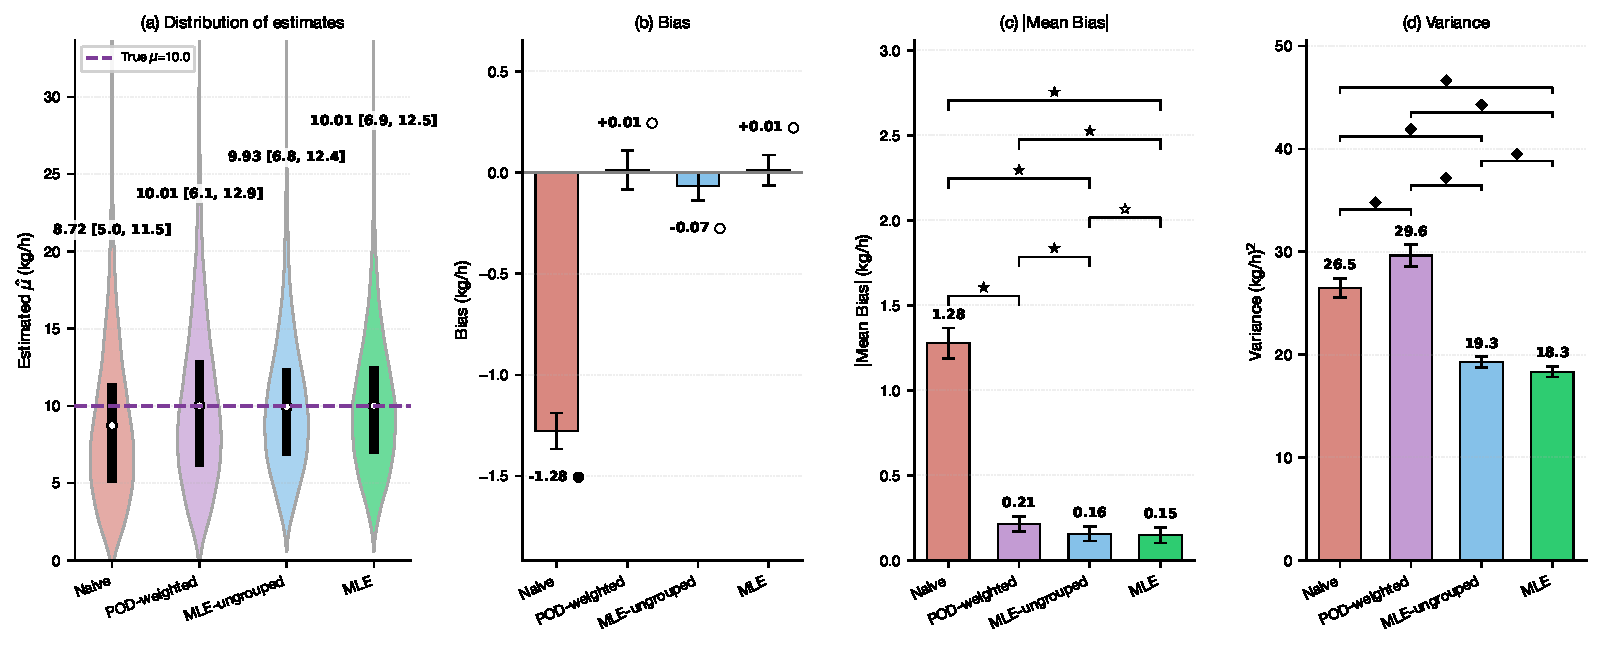
\includegraphics[width=\textwidth]{figures/figure_baseline_violin_v2_wide.pdf}
\caption{Bias--variance comparison of estimation methods ($N = 12{,}500$ simulations, 25 outer batches of 500).
\textbf{(a)}~Violin plots of $\hat{\mu}$; white dots mark the mean, thick bars the interquartile range (IQR), and bold annotations show mean~[IQR]. The dashed line indicates the true value $\mu = 10.0$~kg/h.
\textbf{(b)}~\edit{Signed mean bias (kg/h) for each method, averaged across outer batches.} Filled circles~($\bullet$) indicate the null hypothesis of unbiasedness is rejected at $p < 0.05$ (one-sample $t$-test on 25 batch means); open circles~($\circ$) indicate it cannot be rejected.
\textbf{(c)}~\edit{Absolute value of the signed mean bias, $|\bar{b}|$ (kg/h), averaged over 25 outer batches.} Brackets with filled stars~($\bigstar$) denote pairs whose absolute biases differ significantly ($p < 0.05$, paired $t$-test); open stars~($\star$) indicate no significant difference.
\textbf{(d)}~Variance of $\hat{\mu}$, averaged over 25 outer batches. Brackets with filled diamonds~($\blacklozenge$) denote pairs whose variances differ significantly ($p < 0.05$, paired $t$-test); open diamonds~($\lozenge$) indicate no significant difference.
Error bars in panels (b)--(d) are 95\% confidence intervals from outer-batch replication. \new{Panels (b) and (c) report the same underlying statistic — the mean bias across outer batches — with and without the absolute value: panel (b) preserves sign and supports assessment of systematic over- or under-estimation of $\mu$, while panel (c) reports magnitude and supports pairwise comparison of bias size across methods.} % [EVAN p.8 — "I don't understand the difference between Bias and Mean Bias"]
Full test statistics and exact $p$-values are reported in SI, Section~S7, Tables~S3 and~S4.}
\label{fig:baseline}
\end{figure}

\edit{The naive estimator exhibits substantial bias ($\bar{b} = -1.28$~kg/h, $|\bar{b}| = 1.28$~kg/h), as expected: it discards small undetected emissions entirely. The POD-weighted, MLE-ungrouped, and MLE estimators all correct for this bias. Their mean estimates are 10.01, 9.93, and 10.01~kg/h respectively, against a true value of 10.0~kg/h; the unbiasedness null hypothesis is not rejected for any of the three at $p < 0.05$ (Figure~\ref{fig:baseline}b, open circles). Variances differ markedly: the POD-weighted estimator has variance 29.6~(kg/h)$^2$, the MLE-ungrouped 19.3, and the MLE 18.3, corresponding to a 38\% variance reduction of the MLE relative to the POD-weighted baseline. The pairwise variance differences between the MLE and both the naive and POD-weighted estimators are significant at $p < 0.05$ (Figure~\ref{fig:baseline}d, filled diamonds). The gap between MLE-ungrouped and the full MLE (19.3 vs.\ 18.3) isolates the variance contribution of event-level grouping; the remaining gap from POD-weighted to MLE-ungrouped (29.6 vs.\ 19.3) reflects the value of the HMM treatment of non-detection information.}

\new{The sign and functional form of this variance reduction across monitoring regimes are examined in Section~\ref{sec:sweeps_main}; robustness to misspecification of sensor parameters is characterized in SI, Section~\ref{sec:misspec_SI}.}

\subsubsection{Recovery of Underlying Parameters}

\begin{figure}[htbp]
\centering
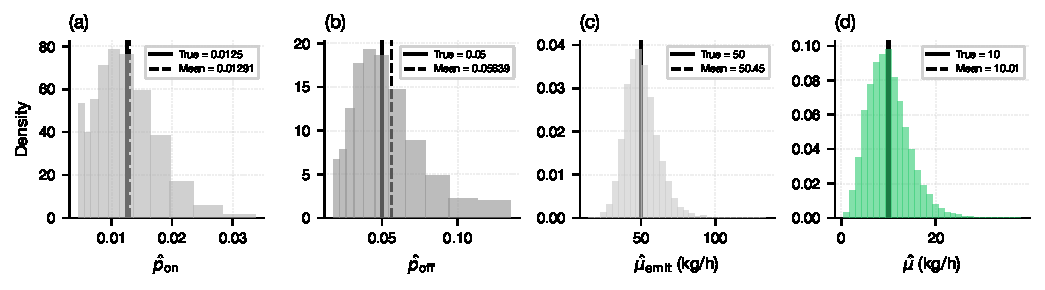
\includegraphics[width=\textwidth]{figures/figure1_histograms.pdf}
\caption{\new{\textbf{(a--d)}~}Distributions of MLE parameter estimates across $N = 12{,}500$ simulations ($25 \times 500$). From left to right: \new{(a)~}ON transition probability~$\hat{p}_{\text{on}}$, \new{(b)~}OFF transition probability~$\hat{p}_{\text{off}}$, \new{(c)~}conditional mean emission rate~$\hat{\mu}_{\text{emit}}$, and \new{(d)~}time-averaged emission rate~$\hat{\mu}$. Solid vertical lines mark the true values; dashed lines mark the sample means. All four parameters are well recovered, with~$\hat{\mu}_{\text{emit}}$ and~$\hat{\mu}$ nearly unbiased and~$(\hat{p}_{\text{on}},\hat{p}_{\text{off}})$ exhibiting small positive shifts\new{ consistent with finite-sample bias rather than model misspecification, as they decrease monotonically with $T$ (SI, Section~\ref{sec:sweep_T})}. % [EVAN p.9/p.11 — finite-sample answer]
}
\label{fig:param_histograms}
\end{figure}

Beyond the aggregate emission rate, our method estimates the underlying model parameters (Figure~\ref{fig:param_histograms}). The individual Markov chain parameters are reasonably well recovered, though with some systematic shifts: $p_{\text{on}}$ is slightly overestimated (true: $0.0125$, estimate: \edit{$0.0129$}) and $p_{\text{off}}$ likewise (true: $0.05$, estimate: \edit{$0.0564$}), \edit{a finite-sample effect characteristic of MLEs at finite $T$ that decreases with campaign length (SI, Section~\ref{sec:sweep_T})}. The conditional mean emission rate $\mu_{\text{emit}}$ is nearly unbiased (true: $50.0$~kg/h, estimate: \edit{$50.45$~kg/h}), indicating that the backward-recursion IPW correction and multi-technology measurement averaging effectively recover the emission size distribution. % [EVAN p.9/p.11 answered again here]

The relative bias of all estimated parameters decreases monotonically with~$T$, and the coefficient of variation narrows as expected. A full composite showing relative bias~(\%) and coefficient of variation (CV,~\%) for each parameter as a function of~$T$ is provided in the SI (Section~S9, Figure~S5).

%-----------------------------------------------------------------------------
\subsection{Sensitivity to Model Parameters}
\label{sec:sweeps_main}
%-----------------------------------------------------------------------------

\edit{We examine how the relative performance of our method varies across the parameter space by conducting systematic sweeps over three key variables: snapshot cadence, emission persistence, and snapshot detection threshold. In each sweep, a single parameter is varied while all others are held at baseline values. Sweeps over continuous-monitoring parameters ($p_{\text{cont}}$ and $T_{\text{cont}}$) are reported in the SI (Sections~\ref{sec:sweep_pcont_SI} and~\ref{sec:sweep_Tcont_SI}), where they complement the main-text analysis by characterizing how continuous-sensor coverage interacts with variance reduction.}

\begin{figure}[htbp]
\centering
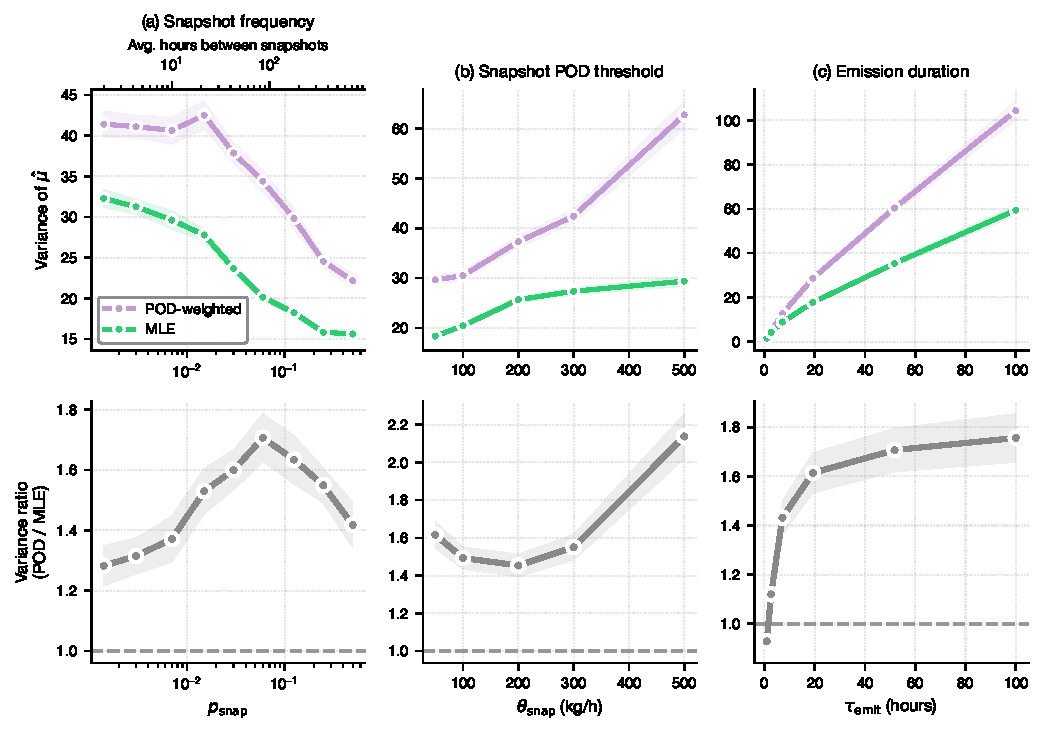
\includegraphics[width=\textwidth]{figures/figure4_composite.pdf}
\caption{Sensitivity of estimation variance to key parameters (shaded bands show 95\% confidence intervals over $25$ replicates). Each column varies one parameter while holding all others at baseline values. Top row: variance of the MLE and POD-weighted estimators. Bottom row: variance ratio (POD-weighted / MLE); values above the dashed line indicate lower MLE variance. \edit{\textbf{(a)}~Snapshot observation probability $p_{\text{snap}}$ (top axis also shown in units of average time between snapshot observations). \textbf{(b)}~Mean emission duration $\tau_{\text{emit}}$. \textbf{(c)}~Snapshot 50\% POD threshold.}} % [EVAN p.11 — add p_snap sweep, report cadence in time-between units]
\label{fig:sweeps}
\end{figure}

% [PB — new p_snap sweep, replacing the p_cont sweep that is moved to SI]
\subsubsection{Snapshot Cadence}
\new{The parameter $p_{\text{snap}}$ controls the frequency of snapshot observations. Figure~\ref{fig:sweeps}a reports estimator variance across a range spanning monthly surveys ($p_{\text{snap}} \approx 0.0014$, corresponding to one observation every approximately 720 hours) through several observations per day ($p_{\text{snap}} = 0.3$). The MLE exhibits lower variance than the POD-weighted estimator at all cadences examined; the variance ratio [BEHAVIOR — describe shape once run]. The precision advantage is preserved even at monthly-survey cadences, which correspond approximately to the upper bound of survey frequency commissioned by commercial operators \citep{[REF]}.}

\subsubsection{Emission Duration}

The mean emission duration $\tau_\text{emit} = 1/p_{\text{off}}$ controls event persistence (Figure~\ref{fig:sweeps}b). The MLE's advantage grows monotonically with $\tau_\text{emit}$: at $\tau_\text{emit} = 100$~hours the variance ratio reaches approximately 1.7. Persistent emissions generate multiple detections from the same event, and the MLE exploits this through plume identification (Step~1), treating them as repeated measurements of one quantity. The POD-weighted estimator treats each detection independently, discarding this information. At very short durations ($\tau_\text{emit} < 3$~hours), consecutive observations rarely sample the same event and the variance ratio approaches 1.0.


\subsubsection{Detection Threshold}

The snapshot threshold $\theta_{\text{snap}}$ controls what fraction of emissions the less sensitive technology can detect (Figure~\ref{fig:sweeps}c). As the threshold worsens, variance increases for both methods, but the MLE degrades more gracefully: the variance ratio exceeds 1.5 at $\theta_{\text{snap}} = 200$~kg/h and reaches 2.4 at $\theta_{\text{snap}} = 500$~kg/h. The MLE explicitly models detection probability, so it recognises that a non-detection from a high-threshold sensor is less informative than one from a low-threshold sensor. The POD-weighted estimator treats all non-detections identically, and its variance therefore grows more steeply as the snapshot sensor becomes less sensitive.

\subsection{Practical Implications}

The variance reduction achieved by our method has direct consequences for monitoring program design. Under standard asymptotic arguments, the number of independent campaigns $N$ required to estimate $\mu$ within $\pm\varepsilon\%$ at 95\% confidence is
\begin{equation}
    N = \left(\frac{1.96}{\varepsilon}\right)^{\!2} \frac{\mathrm{Var}(\hat{\mu})}{\mu^2},
    \label{eq:sample_size}
\end{equation}
so that $N$ scales linearly with estimator variance. Because the MLE reduces variance by approximately \edit{38\%}, it requires \edit{38\%} fewer campaigns at every precision target. Figure~\ref{fig:precision} quantifies this: to estimate the mean within $\pm 3\%$ of the true value, the MLE requires approximately \edit{783} campaigns compared to \edit{1{,}265} for the POD-weighted estimator; at $\pm 5\%$ precision, approximately \edit{282} versus \edit{455}; and at $\pm 10\%$, approximately \edit{70} versus \edit{114}. The shaded bands show the 95\% confidence interval on these numbers, propagated from the experiment-to-experiment variability in the variance estimate.

% [EVAN p.12 — "The largest number of aerial surveys any operator is likely to pay for is 12 per year"]
\new{These sample-size estimates must be interpreted in light of current monitoring economics. For aerial surveys, cost per overflight limits the cadence any single operator is likely to commission for a given facility to approximately twelve per year; meeting the sample-size requirements above at aircraft-only cadences therefore requires pooling across facilities. Satellite observations operate under a different cost structure: tasked revisits carry comparatively low marginal cost, and the baseline cadence of three observations per day is achievable for high-priority facilities under current and near-term constellations. In either case, the variance reduction afforded by the MLE translates into either improved precision at fixed monitoring expenditure or reduced expenditure at a fixed precision target.}

\begin{figure}[htbp]
\centering
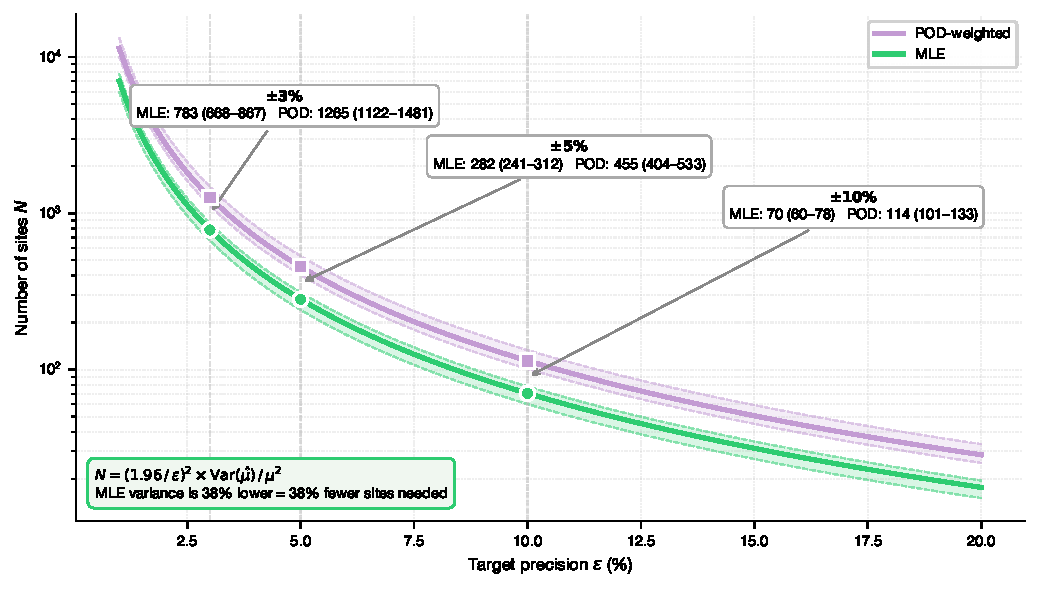
\includegraphics[width=\textwidth]{figures/figure5_precision.pdf}
\caption{Required sample size to estimate~$\mu$ within~$\pm\varepsilon\%$ at 95\% confidence, derived analytically from the single-experiment variance via equation~(\ref{eq:sample_size}). Shaded bands show 95\% confidence intervals from the variability across 25~outer batches. Annotated boxes give the required number of campaigns at three precision targets ($\pm 3\%$, $\pm 5\%$, $\pm 10\%$), with ranges in parentheses. Because variance scales linearly into $N$, the MLE's \edit{38\%} variance reduction translates directly into \edit{38\%} fewer required campaigns at every precision level.}
\label{fig:precision}
\end{figure}

The same variance reduction also improves the ability to detect emission changes over time. In a before--after comparison where $N$ sites are surveyed before and after an intervention, the width of the confidence interval for the change in mean emissions scales with $\sqrt{\mathrm{Var}(\hat{\mu})/N}$. Lower variance therefore means that smaller true changes become statistically distinguishable from zero. Concretely, to reliably detect a 20\% reduction in emissions (with 80\% probability of doing so), the MLE requires approximately \edit{72} sites per group compared to \edit{116} for the POD-weighted estimator. For a fixed monitoring budget, the MLE can resolve emission changes approximately \edit{21\%} smaller than the POD-weighted estimator using the same data.

More broadly, our simulation framework provides variance as a function of the design parameters $(p_{\text{snap}}, p_{\text{cont}}, T_{\text{cont}}, \theta_{\text{snap}})$, which enables principled survey optimization. A monitoring program with a fixed budget can independently choose its snapshot frequency and continuous deployment rate: increasing the continuous monitoring does not mechanically reduce the snapshot survey frequency. This allocation can be framed as minimizing estimator variance subject to a budget constraint, where the cost structure depends on the specific platforms deployed (e.g., satellite tasking versus ground-based sensors). Our results provide the variance surface needed to solve such optimization problems numerically, though the optimal design will depend on site-specific factors: relative technology costs, expected emission persistence, and available infrastructure.


\newpage

\section{Discussion}
\label{sec:discussion}

% [EVAN p.12 — "I suggest adding a paragraph at the beginning of this section that highlights the key high-level takeaways"]
\new{Three conclusions emerge from these results. First, temporal correlation among repeated observations of the same emission source carries information that is discarded by standard estimators; a maximum likelihood framework that explicitly models the latent emission state recovers this information and, in the simulation settings examined here, reduces the variance of the time-averaged emission estimate by approximately 38\% relative to a POD-weighted baseline. Second, these gains are robust across monitoring regimes: they are largest when emissions are persistent and snapshot sensors have relatively high detection thresholds, but remain substantial when cadences are sparse or sensor sensitivity is well matched to the emission-size distribution. Third, the framework is modular in its treatment of sensor characteristics, which enter only as inputs to the likelihood (POD curve, noise model, and cadence); as a result, the same estimator accommodates satellite, aerial, mobile, and fenceline data, either individually or jointly, without structural modification. The remainder of this section examines the assumptions underlying these conclusions and the extensions they suggest.}

Our framework estimates emissions at the spatial scale at which individual measurements are made. For ground-based CMS and aircraft, this is typically a single facility; for satellites, it depends on instrument resolution. \edit{High-resolution instruments (e.g., those with sub-50-m pixel sizes)} can isolate individual facilities, while moderate-resolution instruments may aggregate multiple sources within a single pixel. % [EVAN p.12 — "Why highlight GHGSat here?" — genericized]
The framework applies at whatever scale the instrument resolves: if a pixel contains multiple sources, the estimated rate represents the aggregate and the ON/OFF dynamics reflect whether any source within the pixel is active. Basin-scale estimation then proceeds by aggregating facility-level estimates, propagating uncertainty through the sum.

Several assumptions deserve discussion. The two-state Markov model assumes discrete ON/OFF switching with constant transition probabilities, whereas real emissions may vary continuously and depend on operational factors that change over time. The most consequential violations are likely to be time-of-day or seasonal effects that modulate emission frequency (e.g., tank flashing driven by temperature cycles), since these induce non-stationarity in $p_{\text{on}}$ and $p_{\text{off}}$. When such patterns are regular and known, the analysis window can be restricted to a homogeneous period; when they are unknown, the estimated transition probabilities represent effective averages over the window, and the resulting $\hat{\mu}$ remains a valid time-average provided the observation schedule is not itself correlated with the non-stationarity.

We assume POD curves are known from controlled release experiments~\citep{Sherwin2023, ElAbbadi2024, chen2024comparing, mcmanemin2026controlled}, though in practice detection probability varies with atmospheric conditions, background surface coverage, topographic conditions, and viewing geometry. POD misspecification would propagate into the IPW weights and the HMM emission probabilities. Systematic overestimation of POD would underweight detected events and overcount non-detections as true OFF states, biasing $\hat{\mu}$ downward; the reverse would produce upward bias. The magnitude of this effect depends on how much the true POD deviates from the assumed curve across the emission-size range that contributes most to total flux. \edit{We characterize this sensitivity quantitatively in SI, Section~\ref{sec:misspec_SI}, where we perturb the assumed POD and noise parameters around their true values and report the resulting inflation of total estimator variance; within the range of realistic misspecification, the MLE retains a variance advantage over the POD-weighted baseline.}

\edit{The log-normal assumption for $f$ is used in our simulations but is not essential to the framework.} The estimation procedure requires a parametric form only to compute the marginal detection probability $\kappa$; the IPW correction and HMM steps are otherwise distribution-agnostic. If the true emission-size distribution were heavy-tailed (e.g., Pareto or log-Pareto), the lognormal specification could underestimate $\kappa$ and hence overweight detected events. In practice, the choice of $f$ matters most when detection thresholds are high relative to the bulk of the distribution, so that the shape of the left tail strongly influences $\kappa$. Extending the framework to nonparametric or semi-parametric specifications of $f$ is straightforward in principle but would require additional regularization.

% [EVAN p.12 — "It would be good to discuss survey frequency as a limitation/extension"]
\new{\paragraph{Survey frequency.} The baseline considered here assumes approximately three snapshot observations per day, which approaches the upper bound of currently feasible coordinated deployments; routine single-platform operations are an order of magnitude or more sparser. Estimator variance grows as cadence decreases for any method, and at sufficiently sparse cadences the sample contains too few detected events to identify $p_{\text{on}}$ separately from $\mu_{\text{emit}}$. The $p_{\text{snap}}$ sweep in Section~\ref{sec:sweeps_main} and the very-sparse realization in SI, Section~\ref{sec:sparse_SI} delineate the regime in which the method remains applicable; in sparser regimes, identifiability can be restored by pooling across comparable facilities, or the POD-weighted estimator can be used in its place.}

% [EVAN p.12 — "fenceline continuous monitors have a basically censored error distribution"]
\new{\paragraph{Noise model realism.} The lognormal noise specification in equation~\eqref{eq:noise} captures the approximately scale-invariant relative error observed in controlled-release tests of aerial and satellite platforms. It does not, however, reflect the behavior of fenceline continuous monitors, whose error distributions are typically left-censored: rates below an instrument-specific floor are reported as zero rather than as small positive values. Accommodating such a distribution within the framework requires replacing equation~\eqref{eq:noise} with a censored lognormal. The downstream implications for plume identification, IPW weights, and the HMM forward algorithm merit dedicated treatment and constitute a priority for future work on fenceline applications.}

Natural extensions of this work include multi-state models (e.g., distinguishing low and high emission regimes), hierarchical models that pool information across similar facilities to improve estimates at sparsely observed sites, spatial aggregation frameworks that extend the likelihood to jointly model multiple co-located sources, and sequential updating schemes for real-time operational monitoring.


\section{Conclusion}
\label{sec:conclusion}

We have presented a maximum likelihood framework for estimating time-averaged methane emissions from heterogeneous monitoring data. The method jointly models emission intermittency and size-dependent detection bias, extracting information from both detections and non-detections across technologies with different sensitivities and sampling cadences.

In simulations calibrated to \edit{moderately intensive monitoring scenarios}, the method achieves \edit{38\%} variance reduction relative to POD-weighted estimation under baseline conditions, with gains increasing for persistent emissions observed by complementary sensor types. These reductions translate directly into lower sample-size requirements: for a given precision target, fewer site-visits are needed.

Because sensor characteristics enter as modular inputs, the framework accommodates new instruments without structural changes to the estimator. As the methane monitoring landscape continues to diversify, principled methods for combining these data streams become increasingly important. Our framework provides a statistical foundation for doing so, leveraging the full information content of modern monitoring systems to support accurate, measurement-based emission estimates.

%=============================================================================
\section{Conflicts of Interest}
%=============================================================================

The authors declare no competing interests.

%=============================================================================
\section{Funding}
%=============================================================================

[To be added]

%=============================================================================
\section{Data Availability}
%=============================================================================

The code and simulation configuration files will be made available in a public repository upon publication.

%=============================================================================
\section{Author Contributions}
%=============================================================================

P.B. developed the methodology, designed and ran the simulations, analyzed the results, and wrote the manuscript. E.S. and A.B. provided guidance on methodology and applications and contributed to manuscript revision.

%=============================================================================
\section{Acknowledgments}
%=============================================================================

[To be added]

%=============================================================================
% Bibliography
%=============================================================================
\bibliographystyle{oup-abbrvnat}
\bibliography{references}

\end{document}